\documentclass[11pt,a4paper]{article}

% ---------- Layout: spacious ----------
\usepackage[a4paper, top=3cm, bottom=3cm, left=3.2cm, right=3.2cm]{geometry}
\usepackage{setspace}
\setstretch{1.3}
\usepackage[parfill]{parskip}
\setlength{\parskip}{0.8em}

% ---------- Fonts ----------
\usepackage[T1]{fontenc}
\usepackage{newpxtext,newpxmath}
\usepackage{microtype}

% ---------- Packages ----------
\usepackage{amsmath}
\usepackage{graphicx}
\usepackage{booktabs}
\usepackage{tabularx}
\usepackage{array}
\usepackage{enumitem}
\usepackage{xcolor}
\usepackage{caption}
\usepackage{tikz}
\usetikzlibrary{arrows.meta, positioning, fit, calc, shapes.geometric, backgrounds}
\usepackage{titlesec}
\usepackage{needspace}
\usepackage{placeins}
\usepackage{float}
\usepackage{multirow}
\usepackage[most]{tcolorbox}
\usepackage[colorlinks=true, linkcolor=teal!70!black, urlcolor=teal!70!black, citecolor=teal!70!black]{hyperref}

\graphicspath{{slides/walrus_plan/}{slides/update/}{slides/method/}{slides/squeeze/}{slides/box/}}

\definecolor{teal}{HTML}{13A89E}
\definecolor{ink}{HTML}{1B2B3A}
\definecolor{muted}{HTML}{5A6B7B}
\definecolor{greyc}{HTML}{9AA6B2}
\definecolor{orangec}{HTML}{E05A2B}
\definecolor{purplec}{HTML}{9B7FC0}
\definecolor{navy}{HTML}{232959}

\titleformat{\section}{\needspace{9\baselineskip}\Large\bfseries\color{ink}}{\thesection}{0.8em}{}
\titlespacing*{\section}{0pt}{2.2em}{1.0em}
\titleformat{\subsection}{\needspace{6\baselineskip}\large\bfseries\color{ink}}{\thesubsection}{0.7em}{}
\titlespacing*{\subsection}{0pt}{1.6em}{0.6em}
\titleformat{\subsubsection}{\normalsize\bfseries\color{ink}}{\thesubsubsection}{0.6em}{}
\titlespacing*{\subsubsection}{0pt}{1.2em}{0.4em}

\captionsetup{font={small,stretch=1.15}, labelfont={bf,color=ink}, skip=10pt, margin=0.5cm}
\setlist{itemsep=0.45em, topsep=0.4em, leftmargin=1.6em}

% a quiet box for the main question and key points
\newtcolorbox{keybox}{colback=teal!5, colframe=teal!55, boxrule=0.6pt, arc=3pt, left=12pt, right=12pt, top=8pt, bottom=8pt}
\newtcolorbox{notebox}{colback=gray!4, colframe=greyc, boxrule=0.5pt, arc=3pt, left=12pt, right=12pt, top=7pt, bottom=7pt}

\newcommand{\question}[1]{%
  \vspace{0.4em}\begin{center}\begin{minipage}{0.85\textwidth}\setstretch{1.35}\large\itshape\color{ink}#1\end{minipage}\end{center}\vspace{0.5em}}


\begin{document}

% =====================================================================
% Title
% =====================================================================
\begin{center}
  \vspace*{1.5cm}
  {\LARGE\bfseries\color{ink} What do physics foundation models share inside?\par}
  \vspace{0.8em}
  {\large\color{muted} Looking inside Walrus: do different PDEs use the same parts of the model,\\and is what they share physics?\par}
  \vspace{2em}
  {\normalsize Research plan \quad·\quad Maarten Stork \quad·\quad 28 October 2026\par}
  \vspace{1.5em}
\end{center}

\begin{center}
\begin{minipage}{0.86\textwidth}
\setstretch{1.25}
\small
\textbf{In one paragraph.}
Foundation models for PDEs are trained once on many kinds of physics and then learn new problems faster.
Nobody knows why. One explanation: inside, the model has built something that holds for many equations, a shared core.
The other: it keeps every equation in its own corner, and only generic skills carry over, so it is several models in one box.
We test this inside \emph{Walrus}~\cite{walrus}, a released 1.3-billion-parameter physics foundation model trained on 19 systems.
\textbf{Part A} asks \emph{whether} different PDEs share the inside of the model, with four tests we built and checked on our own
model (neurons, directions, paths, and removing parts). A small \emph{lab model} we can retrain adds what Walrus cannot give:
what happens when the model has no room to keep things apart.
\textbf{Part B}, only where Part A finds sharing, asks \emph{what} is shared: can physical quantities be read out of it,
do they agree with each other the way the laws of physics say, and does the model use them?
On our own small model (Poseidon-T design, 8 PDEs), Part A already gives a clear first answer: the PDEs use the same neurons,
but mostly separately per equation, and not grouped by PDE type. The question now is whether a real, large foundation model does the same.
\end{minipage}
\end{center}

\vspace{1.2em}
\begin{center}
\begin{minipage}{0.86\textwidth}
\small\color{muted}
\textbf{Contents.}\quad
1~The big goal \quad 2~Words we use \quad 3~What we already know \quad 4~Related work \quad 5~The models \quad
6~Part A: is it shared? \quad 7~Part B: is it physics? \quad 8~Order \quad 9~Risks \quad 10~What comes out
\end{minipage}
\end{center}

\newpage
% =====================================================================
\section{The big goal}
% =====================================================================

\subsection{Foundation models for PDEs work, and nobody knows why}

A \emph{foundation model} for PDEs is one large network, trained once on simulations of many kinds of physics:
fluids, waves, chemistry, plasma. Afterwards it learns a new problem from far fewer examples than a model trained from scratch.
Poseidon~\cite{poseidon}, Multiple Physics Pretraining~\cite{mpp} and Walrus~\cite{walrus} all show this.

What these papers do not show is \emph{why}. The model never sees an equation, only fields on a grid.
So what is it that carries over from one kind of physics to another?

This is the question from our supervisor meeting: \emph{is there some shared ``magic'' inside, a physical pattern that helps
for all these equations?} The whole point of one big model for many kinds of physics rests on it.
There are two very different answers (Figure~\ref{fig:stories}).

\begin{itemize}[itemsep=0.7em]
  \item \textbf{Story 1, shared magic.} Inside, the model has built something that holds for many equations:
  for example a common way to handle transport, diffusion or waves. Equations that behave alike
  (the textbook PDE types: elliptic, parabolic, hyperbolic) would then sit together inside.
  That is what justifies one big model for all physics, and that shared part is worth studying: it might be a picture of physics.
  \item \textbf{Story 2, several models in one box.} Inside, every equation keeps to its own part.
  Only generic things are shared: reading a field in, drawing one out, keeping numbers in range.
  Then the case for one big model is weak: it is mainly a convenient package,
  and a few separate, smaller models would make just as much sense.
\end{itemize}

We do not set out to show which design predicts better. We look inside, because that is where the justification for one big model either holds or does not.

\begin{figure}[htbp]
  \centering
  \includegraphics[width=\textwidth]{two_stories.png}
  \caption{The two stories, as a cartoon (not data). Each cloud is the inside activity of one PDE.
  Left: PDEs of the same type sit together, shared magic. Right: every PDE has its own corner.}
  \label{fig:stories}
\end{figure}

\subsection{Why it matters}

\begin{itemize}[itemsep=0.6em]
  \item \textbf{The case for one big model.} If the inside is shared, one model for all physics is well justified.
  If it is several models in one box, that justification is weak, and separate parts per type of physics, or separate smaller models, make as much sense.
  \item \textbf{Trust.} A model that holds a consistent picture of the physics should behave sensibly on new settings.
  A model built from separate shortcuts can fail without warning.
  \item \textbf{Understanding transfer.} Pretraining helps; knowing what is shared tells us what kind of pretraining helps, and why.
\end{itemize}

\subsection{The main question}

\question{Do different PDEs share the inside of a physics foundation model?
And where they do, is what they share a picture of the physics?}

The question has two parts, in this order. The second only makes sense where the first finds something.

\begin{keybox}
\textbf{Part A: is it shared?} Do different PDEs use the same parts of the model, and does the model need those parts?
Are PDEs of the same type grouped together? \hfill Section~\ref{sec:partA}

\vspace{0.4em}
\textbf{Part B: is it physics?} Only where Part A finds sharing.
Can physical quantities be read out of the shared part, do they agree with each other through the laws of physics,
and does the model use them? \hfill Section~\ref{sec:partB}
\end{keybox}

\textbf{Careful: shared is not yet physics.} A shared part can be generic: smoothing, taking differences, keeping numbers in range.
That is useful for every PDE, but it is not a picture of the physics. Sharing is the precondition; Part B decides.
And the other way round: if Part A finds every PDE in its own corner, that is itself the answer (story 2), and an interesting one.

\begin{figure}[htbp]
\centering
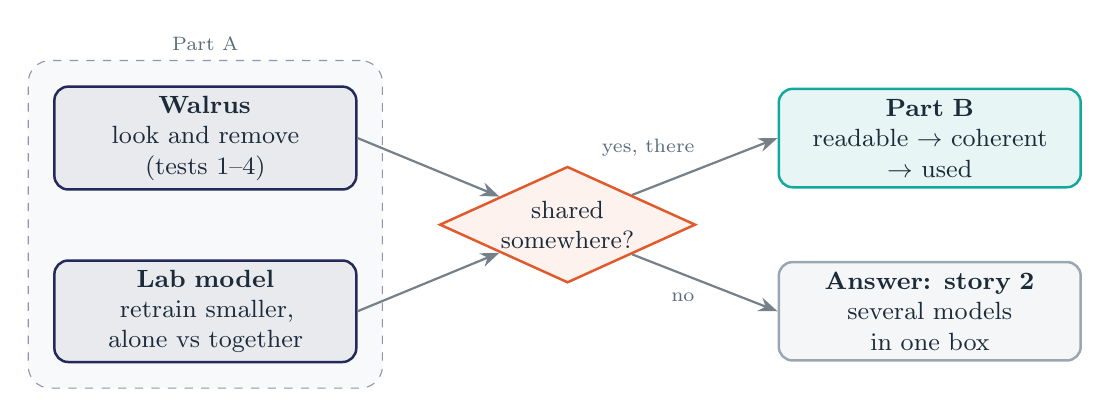
\begin{tikzpicture}[
  box/.style={draw=#1, fill=#1!10, rounded corners=5pt, line width=0.9pt, minimum height=1.25cm, text width=3.6cm, align=center, font=\small, text=ink},
  box/.default=teal,
  dec/.style={draw=orangec, fill=orangec!8, diamond, aspect=2.2, line width=0.9pt, align=center, font=\small, text=ink, inner sep=1pt},
  arr/.style={-{Stealth[length=2.4mm]}, line width=0.8pt, color=ink!60},
  lab/.style={font=\scriptsize, color=muted},
]
  \node[box=navy] (walrus) at (0, 0) {\textbf{Walrus}\\look and remove\\(tests 1--4)};
  \node[box=navy] (lab)    at (0, -2.2) {\textbf{Lab model}\\retrain smaller,\\alone vs together};
  \node[dec] (d) at (4.6, -1.1) {shared\\somewhere?};
  \node[box=teal] (B) at (9.2, 0) {\textbf{Part B}\\readable $\to$ coherent\\$\to$ used};
  \node[box=greyc] (no) at (9.2, -2.2) {\textbf{Answer: story 2}\\several models\\in one box};
  \begin{scope}[on background layer]
    \node[draw=navy!50, dashed, fill=navy!3, rounded corners=8pt, inner sep=9pt, fit=(walrus)(lab), label={[lab]above:Part A}] {};
  \end{scope}
  \draw[arr] (walrus.east) -- (d);
  \draw[arr] (lab.east) -- (d);
  \draw[arr] (d.north east) -- node[lab, above left] {yes, there} (B.west);
  \draw[arr] (d.south east) -- node[lab, below left] {no} (no.west);
\end{tikzpicture}
\caption{The plan in one picture. Part A looks inside Walrus and experiments on a small lab model.
What it finds decides whether, and where, Part B looks for physics.}
\label{fig:plan}
\end{figure}

% =====================================================================
\section{Words we use}
% =====================================================================

\begin{notebox}
\setlength{\parskip}{0.55em}
\textbf{PDE type.} The textbook sorting of PDEs by how information travels.
\emph{Elliptic}: a steady state, every point depends on all others at once (Poisson, Helmholtz).
\emph{Parabolic}: spreads and smooths over time (heat, reaction--diffusion).
\emph{Hyperbolic}: travels at a finite speed and stays sharp (waves, compressible gas).
Some, like the incompressible Navier--Stokes equations, are \emph{mixed}.

\textbf{System.} One dataset: one equation in one setting (for example compressible Euler with periodic walls).
Two systems can share an equation.

\textbf{Layer} (in Walrus: \emph{block}). One step of the network. Walrus has 40 of them, all the same shape.

\textbf{Patch, token.} The model cuts the field into small squares. Each becomes a list of numbers that travels through the layers.

\textbf{Neuron, activation.} Inside each layer, a small network (the MLP) computes many numbers per patch.
Each of those is a neuron; its value for one patch is its activation.

\textbf{Direction.} A fixed mix of neurons. A PDE's \emph{directions} in a layer are the mixes along which its activations vary most
(principal components). Two PDEs can use the same neurons in different mixes, so directions say more than neurons.

\textbf{Removal.} Changing the inside of the model while it runs (switching off neurons, or taking out directions)
and measuring how much worse each PDE gets. This tests whether the model \emph{needs} a part, not only whether it is active.

\textbf{Probe, readout.} A simple formula (a weighted sum of activations) trained to read a quantity, like kinetic energy,
out of a layer. If a simple formula can do it, the quantity is in there.
\end{notebox}

% =====================================================================
\section{What we already know: our own model}
\label{sec:known}
% =====================================================================

Before turning to Walrus, we built and tested the whole toolkit on a model of our own.
It already gives a clear first answer to Part A, and it taught us what to watch out for.

\subsection{The setup}

We trained one model, \emph{joint2}, with Poseidon-T's design~\cite{poseidon}
(a transformer shaped like a U, 32 layers, about 21 million parameters) and Poseidon's training recipe, from scratch,
on 8 datasets from Poseidon's collection: Poisson and Helmholtz (elliptic), Allen--Cahn (parabolic),
two wave datasets and two compressible Euler datasets (hyperbolic), and incompressible Navier--Stokes (mixed).
It predicts all eight well (test errors 0.9\% to 11.8\%). Then we froze it and looked inside.

\subsection{Four tests}

\begin{enumerate}[itemsep=0.8em]
  \item \textbf{Neurons.} Which neurons does each PDE use? \emph{Result:} every PDE uses almost all of them.
  At most 0.8\% of any layer is used by one type only. Counted neuron by neuron, everything is shared.

  \item \textbf{Directions.} Per PDE and layer, the directions that hold 90\% of its activity (principal components),
  and the overlap between two PDEs' directions~\cite{hu2021lora, chang2022}:
  \begin{equation*}
    \varphi(d, e) = \frac{\lVert U_d^{\top} U_e \rVert_F^{2}}{\min(k_d,\, k_e)}
  \end{equation*}
  where $U_d$ holds PDE $d$'s $k_d$ directions as columns (each of length 1). $\varphi = 1$: the same directions; $\varphi = 0$: at right angles.
  \emph{Result:} at the start and end of the model the PDEs overlap (about 0.6); in the middle, where the solving happens,
  much less (0.14--0.22) (Figure~\ref{fig:known}, left). The middle works like several models side by side.

  \item \textbf{Removal.} Take one PDE's directions out of the middle layers while the model runs
  (after~\cite{saha2026}), and measure every PDE's error:
  \begin{equation*}
    a' = a - U_d U_d^{\top} (a - \mu)
  \end{equation*}
  where $a$ is a patch's activations and $\mu$ the average of the PDE that patch belongs to, so only variation along $U_d$ is removed.
  Control: random directions of the same number.
  \emph{Result:} Poisson, Helmholtz and Euler each break mostly when their \emph{own} directions are removed (Figure~\ref{fig:known}, right).
  The two datasets of one equation hurt each other.

  \item \textbf{Paths.} Which neurons does each PDE's prediction depend on? Importance of neuron $i$ for PDE $d$:
  activation times gradient~\cite{dhamdhere2019}, summed over patches; a PDE's top 10\% is its path.
  \emph{Result:} two PDEs share about 20\% of their paths (two unrelated lists: 10\%; the same model with random weights: 44\%).
  Only the two wave datasets share theirs (71\%).
\end{enumerate}

And a fifth, \textbf{pruning}: deleting neurons outright. Deleting one PDE's top neurons hurts mostly that PDE
(for Poisson, Helmholtz and Euler); deleting the least important 90\% of the middle leaves Allen--Cahn, the waves and Navier--Stokes
almost untouched, while Poisson, Helmholtz and Euler break (Figure~\ref{fig:prune}).

\begin{figure}[htbp]
  \centering
  \includegraphics[width=0.48\textwidth]{c1_overlap.png}\hfill
  \includegraphics[width=0.47\textwidth]{ladder_13-20.png}
  \caption{joint2, real results. Left: overlap of directions per layer, averaged over all 28 pairs of PDEs.
  The middle (grey) is where the PDEs share least. Right: removal in layers 13--20. Row: whose directions are removed;
  column: whose error rises (\% of its normal error). Read per column: the darkest cell is the removal that hurts that PDE most;
  the orange boxes mark the PDE's own directions.}
  \label{fig:known}
\end{figure}

\begin{figure}[htbp]
  \centering
  \includegraphics[width=\textwidth]{prune_overall_13-20.png}
  \caption{joint2, real results. Deleting more and more of the middle, least important neurons first (solid) or random ones (dashed grey).
  Some PDEs barely need the middle; Poisson, Helmholtz and Euler do.}
  \label{fig:prune}
\end{figure}

\subsection{What it says, and what it does not}

\begin{keybox}
\textbf{In joint2: the same neurons, used mostly separately per equation in the middle.}
Sharing follows the \emph{equation} (the two waves, the two Euler sets), not the PDE \emph{type}:
two different hyperbolic equations (wave and Euler) overlap no more than an elliptic and a hyperbolic one (Figure~\ref{fig:groups}).
\end{keybox}

\begin{figure}[htbp]
  \centering
  \includegraphics[width=0.85\textwidth]{groups.png}
  \caption{joint2, real results. Overlap of directions by kind of pair. In the middle, two datasets of the \emph{same equation}
  overlap (0.49), but two equations of the \emph{same type} overlap no more than two of different types (0.12 vs 0.15).}
  \label{fig:groups}
\end{figure}

\textbf{Why this is not the end of the story.}
\begin{itemize}[itemsep=0.6em]
  \item \textbf{Small model, few PDEs.} 21 million parameters, 8 datasets, one parabolic. Real foundation models are 50 times bigger
  and trained on far more physics. Sharing could appear only at that scale.
  \item \textbf{Room to spare.} All 8 PDEs together use only 316--761 of the 1,536 possible directions in a middle layer
  (Figure~\ref{fig:room}). Keeping them apart cost the model nothing. Whether they would share \emph{if they had to} is open.
  \item \textbf{The U shape.} Poseidon's skips carry information around the middle. Some PDEs (Allen--Cahn, waves, Navier--Stokes)
  barely needed the middle at all, which made several results hard to read.
\end{itemize}

\begin{figure}[htbp]
  \centering
  \includegraphics[width=0.85\textwidth]{room.png}
  \caption{joint2, real results. Directions needed by all 8 PDEs together (stacked, coloured by type) per middle layer,
  against the 1,536 neurons available. There is plenty of room for every PDE to have its own corner.}
  \label{fig:room}
\end{figure}

\subsection{Lessons we take along}

\begin{enumerate}[itemsep=0.6em]
  \item \textbf{Neurons alone mislead.} Everything looks shared at the level of neurons. Directions and paths are needed.
  \item \textbf{Read removal results per column.} Some PDEs are fragile (Euler breaks from almost anything, even random removals),
  so a row can look large for the wrong reason. Per column: which removal hurts \emph{this} PDE most?
  \item \textbf{Always a control.} Random weights for the measures, random directions or neurons for removal.
  The trained model must differ from them.
  \item \textbf{Removing variation is not deleting.} Taking out a PDE's directions keeps each neuron's average level; deleting a neuron sets it to 0.
  The two gave very different answers for Allen--Cahn and the waves (they rely on a few very active neurons staying on).
  \item \textbf{Do not change the design to test it.} To squeeze the model, we first removed Poseidon's skips. But then the result is
  about a different model. Squeezing should keep the design and only make it smaller (fewer neurons).
\end{enumerate}

% =====================================================================
\section{Related work}
% =====================================================================

Looking inside neural networks started with language models; it reached physics foundation models in 2025--2026.
A few studies look inside Walrus or Poseidon. None of them asks how much of the model different PDEs share.

\begin{table}[htbp]
\centering
\renewcommand{\arraystretch}{1.55}
\small
\begin{tabularx}{\textwidth}{>{\raggedright\arraybackslash}p{3.6cm} >{\raggedright\arraybackslash}X >{\raggedright\arraybackslash}p{3.6cm}}
\toprule
\textbf{Study} & \textbf{What they did} & \textbf{What is left open} \\
\midrule
Physics Steering~\cite{fear2025} (Walrus) & A ``vortex'' direction found in shear flow, added to the last layer, also adds swirls in other systems.
  & a few hand-picked concepts, one layer, no random control; how much is shared stays open \\
Sparse probes and murky physics~\cite{rosenfeld2026} (Walrus) & Sparse autoencoder features in one layer, on shear flow.
  Some features recur, but do not map cleanly onto known physics. & one system; not across PDEs \\
Liao \& Cao~\cite{liao2026} (Poseidon) & Energy can be read out of Poseidon, but the model does not use it for its predictions.
  & one quantity; readable is not used \\
pADAM~\cite{padam} & Attention patterns suggest one multi-physics model reuses and combines diffusion and advection features.
  & one model, attention only, no removal test \\
Multi-physics papers~\cite{mpp, unsupadapt} & \emph{Claim} a shared representation across physical systems. & not tested inside \\
Vafa et al.~\cite{vafa} & A model that predicts orbits well has not learned Newton's law: its implied forces are nonsense.
  & physics of planets, not PDEs \\
\bottomrule
\end{tabularx}
\caption{The closest work. Our methods come from language models (directions~\cite{chang2022}, removal~\cite{saha2026})
and attribution (paths~\cite{dhamdhere2019, dreyer2024}).}
\end{table}

\textbf{The gap.} Physics Steering shows that \emph{some} concepts transfer between systems in Walrus.
Nobody has measured \emph{how much} of a physics foundation model different PDEs share, \emph{where} in the network,
whether that follows the PDE types, and whether the model \emph{needs} what is shared.
And the step after that, checking whether several read-out quantities agree with each other through the laws of physics,
has, as far as we found, not been done for any physics model.

% =====================================================================
\section{The models}
% =====================================================================

\subsection{The main model: Walrus}

Walrus~\cite{walrus} is a transformer of 1.3 billion parameters, released with its code and weights.
It was trained on 19 systems from The Well~\cite{thewell} and FlowBench: fluids, acoustics, chemistry, astrophysics, plasma, in 2D and 3D.
Given the last 6 snapshots of a system, it predicts the next one (Figure~\ref{fig:walrus}).

\begin{figure}[htbp]
\centering
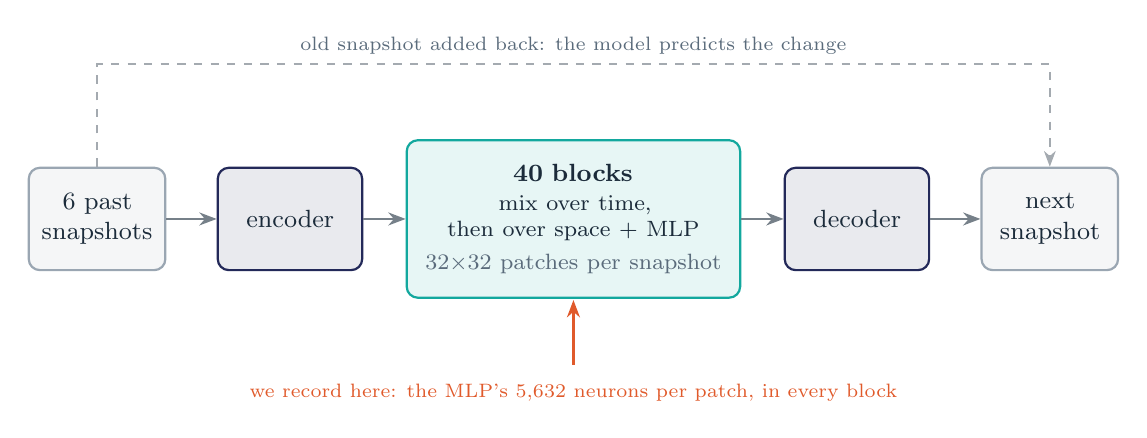
\begin{tikzpicture}[
  b/.style={draw=#1, fill=#1!10, rounded corners=4pt, line width=0.8pt, minimum height=1.3cm, align=center, font=\small, text=ink},
  b/.default=navy,
  arr/.style={-{Stealth[length=2.2mm]}, line width=0.8pt, color=ink!60},
  lab/.style={font=\scriptsize, color=muted, align=center},
]
  \node[b=greyc, text width=1.5cm] (in) at (0,0) {6 past\\snapshots};
  \node[b, text width=1.6cm] (enc) at (2.45,0) {encoder};
  \node[b=teal, text width=4.0cm, minimum height=2.0cm] (blk) at (6.05,0) {\textbf{40 blocks}\\[1pt]{\footnotesize mix over time,\\then over space + MLP\\[1pt]\color{muted}32$\times$32 patches per snapshot}};
  \node[b, text width=1.6cm] (dec) at (9.65,0) {decoder};
  \node[b=greyc, text width=1.5cm] (out) at (12.1,0) {next\\snapshot};
  \draw[arr] (in) -- (enc); \draw[arr] (enc) -- (blk); \draw[arr] (blk) -- (dec); \draw[arr] (dec) -- (out);
  \draw[arr, orangec] (6.05, -1.85) -- (6.05, -1.03);
  \node[lab, text=orangec] at (6.05, -2.2) {we record here: the MLP's 5,632 neurons per patch, in every block};
  \draw[line width=0.7pt, color=ink!40, dashed, -{Stealth[length=2mm]}] (in.north) -- ++(0,1.3) -| node[lab, pos=0.25, above] {old snapshot added back: the model predicts the change} (out.north);
\end{tikzpicture}
\caption{Walrus, simplified (sizes from~\cite{walrus}, Table 3). All 40 blocks work on the same grid of patches
($32 \times 32$ for 2D data); there are no skips around the middle. Each block mixes over time (the 6 snapshots) and over space;
its MLP has 5,632 neurons per patch, which is what we record. The model predicts the change from the last snapshot.}
\label{fig:walrus}
\end{figure}

\textbf{Why Walrus.}
\begin{itemize}[itemsep=0.6em]
  \item \textbf{A real foundation model.} Large, trained on many kinds of physics, among the best on its benchmarks~\cite{walrus}.
  Findings on it say something about physics foundation models, not about one small model.
  \item \textbf{Easy to look inside.} Unlike Poseidon, Walrus is not a U: all 40 blocks have the same shape and nothing goes around them.
  ``The middle'' is not a special place, every block can be compared with every other, and removal cannot be bypassed.
  \item \textbf{Released and studied.} Weights and code are public, and two studies looked inside it~\cite{fear2025, rosenfeld2026}:
  we can compare with them.
  \item \textbf{We only need to run it.} Everything in Part A and Part B uses the frozen model: recording, removal, readouts.
  A 1.3-billion-parameter model fits on one GPU of the DAIC cluster for this.
\end{itemize}

\textbf{What it lacks.} Every Walrus system evolves in time, so there is no clean steady elliptic problem like Poisson.
The Helmholtz staircase comes closest (an elliptic equation, shown oscillating in time). Elliptic PDEs can be added later
by fine-tuning (Section~\ref{sec:elliptic}).

\subsection{The systems we use}

Eight 2D systems, chosen like our own eight: several types, and pairs of the same equation in different settings,
so we can tell ``same equation'' from ``same type'' (the lesson of Figure~\ref{fig:groups}).

\begin{table}[htbp]
\centering
\renewcommand{\arraystretch}{1.5}
\small
\begin{tabularx}{\textwidth}{>{\raggedright\arraybackslash}p{4.3cm} >{\raggedright\arraybackslash}X l l}
\toprule
\textbf{System (The Well)} & \textbf{Equation} & \textbf{Type} & \textbf{Pair} \\
\midrule
acoustic scattering, inclusions & wave equation, medium with inclusions & hyperbolic & \multirow{2}{*}{same equation} \\
acoustic scattering, discontinuous & wave equation, medium with a jump & hyperbolic & \\
Euler multi-quadrants, periodic & compressible Euler (gas, shocks) & hyperbolic & \multirow{2}{*}{same equation} \\
Euler multi-quadrants, open & compressible Euler, open walls & hyperbolic & \\
Gray--Scott & reaction--diffusion (two chemicals) & parabolic & \\
shear flow & incompressible Navier--Stokes & mixed & \multirow{2}{*}{same family} \\
Rayleigh--B\'enard & Navier--Stokes plus heat (convection) & mixed & \\
Helmholtz staircase & Helmholtz, time-harmonic waves & elliptic in space & borderline \\
\bottomrule
\end{tabularx}
\caption{The eight Walrus systems for Part A, all in Walrus's pretraining data (\cite{walrus}, Table 6).
Possible extras: shallow water on the globe (hyperbolic), active matter. 3D systems are left out to keep things comparable.}
\label{tab:systems}
\end{table}

We do not need The Well's terabytes: a few dozen test trajectories per system are enough to record the inside of the model.

\subsection{The lab model}

Walrus cannot be retrained: it was trained on 96 H100 GPUs~\cite{walrus}. Some questions need retraining, such as
``what if the model had less room?'' or ``what if it saw one system only?''. For those we use a small model we train ourselves.

Two candidates, same role:
\begin{itemize}[itemsep=0.6em]
  \item \textbf{Poseidon-T design (joint2).} Ready now: data, training code and all four tests exist, and the first results are in.
  But a different design from Walrus (a U with skips).
  \item \textbf{A mini-Walrus.} Walrus's own code with much smaller settings, trained on a few of the systems above.
  Same design as the main model, so results compare directly. Costs setup and some days of training.
\end{itemize}
\textbf{Plan:} start the lab work on the Poseidon-T design, since it is ready. Move to a mini-Walrus if Part A shows that Walrus
behaves differently from joint2, because then the design matters and the lab model should match it.

% =====================================================================
\section{Part A: is it shared?}
\label{sec:partA}
% =====================================================================

\question{Do different PDEs use the same parts of Walrus, does Walrus need those parts,
and does the sharing follow the PDE types or the equations?}

Part A runs the four tests of Section~\ref{sec:known} on Walrus, step by step, then adds the lab experiments.

\subsection*{Step A0: get Walrus running}

\begin{enumerate}[itemsep=0.5em]
  \item Install Walrus's code and weights on DAIC; download a few dozen test trajectories of each system in Table~\ref{tab:systems}.
  \item \textbf{Sanity check:} reproduce Walrus's own one-step errors on these systems~\cite{walrus}. If we cannot,
  something in our setup is wrong (normalisation, time step, field order), and nothing after this counts.
  \item Make the control: the same architecture with random weights.
\end{enumerate}

\subsection*{Step A1: record the inside}

Freeze Walrus and run every system's test examples through it. In every block, record the MLP's neurons
(the 5,632 numbers per patch inside its MLP, after the gate of its SwiGLU; the equivalent of what we recorded in joint2), for the newest snapshot only.
Keep a random sample of patches per example, as for joint2. The same for the random-weight copy.

\textbf{Watch out:} Walrus reads each system through its own first projection (systems have different fields).
So the first blocks can tell systems apart from the input format alone. What matters is how the tests change \emph{deeper in}.

\subsection*{Step A2: neurons}

Per system and block: the share of neurons that are used (average $|$activation$|$ above 1\% of the block's average).
Neurons used by one system only, by one type only, by all.
\emph{Expected, from joint2:} almost everything used by everyone. This is the baseline that the next steps look beneath.

\subsection*{Step A3: directions}

Per system and block: the principal components that hold 90\% of its activity, and the overlap $\varphi$ between every pair of systems.
Three summaries:
\begin{enumerate}[itemsep=0.5em]
  \item \textbf{Overlap per block}, averaged over pairs, from block 1 to 40 (like Figure~\ref{fig:known}, left).
  Where is Walrus shared, and where split?
  \item \textbf{By kind of pair:} same equation (acoustics--acoustics, Euler--Euler), same family (shear flow--Rayleigh--B\'enard),
  same type but different equation (acoustics--Euler), different type (like Figure~\ref{fig:groups}).
  This is the direct test of ``grouped by type''.
  \item \textbf{Room:} the number of directions all systems need together, against the 5,632 available (like Figure~\ref{fig:room}).
  Does Walrus have room to spare too?
\end{enumerate}
Control: random weights. Overlap in a trained block must differ from the random-weight block to mean anything.

\subsection*{Step A4: paths}

Per system and block: the importance of every neuron for the system's prediction (activation times gradient~\cite{dhamdhere2019}):
\begin{equation*}
  I_{d,i} = \Bigl|\, \sum_{p} a_{p,i}\, \frac{\partial F_d}{\partial a_{p,i}} \,\Bigr|
\end{equation*}
where $a_{p,i}$ is neuron $i$'s activation in patch $p$, and $F_d$ measures system $d$'s prediction.
A system's top 10\% most important neurons is its path through that block. Two systems share a share of their paths;
two unrelated lists share 10\%, the random-weight model sets the other reference.
This needs gradients, so it is the most expensive step, but still one run per system.

\subsection*{Step A5: removal and pruning}

The step that tests whether the model \emph{needs} what it shares.
\begin{enumerate}[itemsep=0.5em]
  \item \textbf{Remove a system's directions} in a range of blocks while Walrus runs, and measure every system's error.
  Read per column. Control: random directions.
  \item \textbf{Delete a system's top neurons} (its path), and measure every system's error. Control: random neurons.
  \item \textbf{Delete more and more}, least important first: which systems break first?
\end{enumerate}
Walrus has no skips, so a removal cannot be bypassed: one of the problems we had with joint2 is gone.
Both kinds of removal (directions, which keep the average level, and deleting, which does not) are reported, because they can differ.

\subsection*{Step A6: the lab experiments}

What Walrus cannot tell us: \emph{does it share when it has to?}
On the lab model, keeping its design and only changing its size (fewer neurons per layer):

\begin{enumerate}[itemsep=0.6em]
  \item \textbf{Squeeze.} Train with fewer and fewer neurons (for the Poseidon-T design: 1,536, 384, 96, 24 in the middle layers),
  for system A alone, system B alone, and A and B together. Find the smallest size that still works for each.
  If together needs about the sum of the two, they are separate; if about the bigger one, they share (Figure~\ref{fig:lab}).
  A natural first pair: Poisson and Euler, two different types that both really use the middle.
  \item \textbf{Does sharing appear?} Run the direction test on each squeezed model. If overlap rises as the room shrinks,
  the PDEs \emph{can} share, they just do not when they do not have to.
\end{enumerate}

\begin{figure}[htbp]
  \centering
  \includegraphics[width=0.85\textwidth]{lab_sizes.png}
  \caption{How the squeeze is read (made-up numbers). The smallest model that still works for each system alone,
  and for both together. Needing the sum means two separate things in one box; fitting in about the bigger one means they share.}
  \label{fig:lab}
\end{figure}

Every run trains from scratch with the full recipe, so this is the expensive part of Part A (about a day per run on DAIC
for the Poseidon-T design; fewer neurons train faster).

\needspace{10\baselineskip}
\subsection*{What Part A can give}

\begin{table}[H]
\centering
\renewcommand{\arraystretch}{1.55}
\small
\begin{tabularx}{\textwidth}{>{\raggedright\arraybackslash}p{4.6cm} >{\raggedright\arraybackslash}X}
\toprule
\textbf{If we see} & \textbf{It means} \\
\midrule
High overlap between types deep in Walrus, shared paths, removals that hurt several types & shared magic: story 1, and one big model is justified. On to Part B, in those blocks. \\
Overlap within a type clearly above between types & grouped by type: the textbook classification exists inside. On to Part B per type. \\
Sharing only within an equation (as in joint2) & several models in one box, organised by equation: story 2, now for a large model. The case for one big model is weak. \\
Shared in some blocks, split in others & a map of where the model shares: Part B on the shared blocks only. \\
Lab: together fits in the bigger one; overlap rises when squeezed & the PDEs \emph{can} share; separation in large models is a luxury of room. \\
\bottomrule
\end{tabularx}
\end{table}

Every row is a finding. Since joint2 showed story 2, finding story 1 in Walrus would be the more surprising result,
and finding story 2 again would show it is not a small-model accident.

% =====================================================================
\section{Part B: is what is shared physics?}
\label{sec:partB}
% =====================================================================

\question{Where Part A finds sharing: does the shared part hold physical quantities,
do they agree with each other the way the laws of physics say, and does the model use them?}

Part B starts only after Part A, and only in the blocks and systems where Part A found sharing.
If Part A finds every system in its own corner, Part B shrinks to one system, as a smaller follow-up.

Three properties, tested in this order. Each can stop the line.

\begin{keybox}
\textbf{1. Readable.} A simple formula can read physical quantities out of the shared part.\\[0.3em]
\textbf{2. Coherent.} Those read-out quantities agree with each other, the way the laws of physics say they must.\\[0.3em]
\textbf{3. Used.} The model relies on them: changing them inside changes its prediction the way physics says.
\end{keybox}

Others have tested 1 (and recently 3) for single quantities~\cite{liao2026, fear2025}. Property 2 is new.

\subsection*{Step B1: readable}

\textbf{How.} Take the activations of one block. Fit a \emph{linear} readout: a weighted sum of the activations that predicts a
physical quantity at every patch. Train it on some simulation runs, test it on others (snapshots of one run look alike,
so mixing them would let the readout memorise).

\textbf{Why only linear.} A weighted sum cannot multiply. If a quantity needs multiplying fields together
(kinetic energy $\tfrac12 \rho |u|^2$ needs speed times speed), a linear readout can only find it if the model has already computed it.
So we choose \emph{hard} quantities: ones that are not a weighted sum of the input. Easy ones prove nothing.

\begin{table}[H]
\centering
\renewcommand{\arraystretch}{1.5}
\small
\begin{tabularx}{\textwidth}{>{\raggedright\arraybackslash}p{3.3cm} >{\raggedright\arraybackslash}X >{\raggedright\arraybackslash}p{3.8cm}}
\toprule
\textbf{System} & \textbf{Hard quantities (never given to Walrus)} & \textbf{Shared with} \\
\midrule
compressible Euler & kinetic energy $\tfrac12 \rho |u|^2$; total energy; Mach number & kinetic energy: all flows \\
shear flow & kinetic energy $\tfrac12 |u|^2$; how fast the flow is sheared $|\nabla u|^2$ & kinetic energy \\
Rayleigh--B\'enard & kinetic energy; heat carried up by the flow $w \cdot b$ & kinetic energy \\
acoustics & acoustic energy (pressure squared plus speed squared) & energy-like \\
Gray--Scott & reaction rate $A B^2$ & --- \\
\bottomrule
\end{tabularx}
\caption{Candidate quantities. All need multiplying fields, so a linear readout of the raw input cannot produce them.
($w$: upward velocity, $b$: temperature, $A, B$: the two chemicals.)}
\end{table}

\textbf{The bridge to Part A: one readout for many systems.} Kinetic energy exists in Euler, shear flow and Rayleigh--B\'enard.
Train the kinetic-energy readout on Euler, and test it, unchanged, on shear flow and Rayleigh--B\'enard.
If one direction reads kinetic energy in all three, the model has one shared concept of it.
This is where ``shared'' (Part A) and ``physics'' (Part B) meet.

\textbf{Controls.}
\begin{itemize}[itemsep=0.4em]
  \item \textbf{The input itself:} a readout straight from the input fields. If it already works, the quantity is too easy.
  \item \textbf{Random weights:} the same readout on the random-weight Walrus.
  \item \textbf{Other blocks:} the same readout in every block, to see where the quantity appears.
\end{itemize}

\subsection*{Step B2: coherent}

\textbf{The idea.} Imagine two models whose readouts are all about equally accurate.
\begin{itemize}[itemsep=0.4em]
  \item The first has a separate shortcut per quantity. Each readout looks fine, but their errors are unrelated,
  so together they break physics.
  \item The second has one picture of the world and reads everything from it. When it is wrong, everything is wrong in the same way:
  it describes one slightly wrong world in which the laws still hold.
\end{itemize}
Single readouts cannot tell these apart. Whether the errors hang together can (Figure~\ref{fig:shuffle}).

\begin{figure}[htbp]
  \centering
  \includegraphics[width=0.75\textwidth]{shuffle.png}
  \caption{How we see whether errors hang together (sketch). Each dot is one example: the error of readout 1 against that of readout 2.
  Left: the errors go together. Right: the same errors, each paired with a random other example; the link is gone.}
  \label{fig:shuffle}
\end{figure}

\textbf{The score, fixed before we measure.} Put the readouts into a law of physics and measure how far off the law is.
Then the same with the errors shuffled between examples, which breaks any link on purpose:
\begin{equation*}
  C = \frac{\text{how far off the law, with shuffled errors}}{\text{how far off the law, with the real readouts}}
\end{equation*}
$C \approx 1$: the real errors break the law as much as unrelated errors, so there is no shared picture.
$C \gg 1$: the errors fit the law much better than chance, so they hang together.

\textbf{Two laws to start with.}
\begin{enumerate}[itemsep=0.6em]
  \item \textbf{Energy in a gas (Euler).} Total energy is internal energy plus kinetic energy:
  $E = \dfrac{p}{\gamma - 1} + \tfrac12 \rho |u|^2$, with $p$ the pressure and $\gamma$ a fixed number of the gas.
  Read out $E$ and the kinetic energy separately; does their difference match the pressure term? No derivatives needed.
  \item \textbf{Heat budget of a slab (Rayleigh--B\'enard).} Take a horizontal band of the fluid. The heat in it changes only through
  its top and bottom edges: conducted, and carried by the flow ($w \cdot b$, read out). The change itself comes from Walrus's own prediction.
  Does the read-out transport add up to the change the model predicts?
\end{enumerate}
Slopes of read-out fields are noisy, so we never take them directly: the laws are checked as averages over smooth regions,
with every slope moved onto a smooth bump we draw ourselves.

\textbf{The comparison that counts:} trained Walrus against random-weight Walrus. Readouts from one block share their input,
so even random weights give some linked errors. Walrus must clearly beat that.

\subsection*{Step B3: used}

A quantity can be readable without the model using it~\cite{liao2026}. So we change it inside and watch what follows.
\begin{enumerate}[itemsep=0.5em]
  \item Take the readout's direction (for example ``more kinetic energy'', or ``more heat carried up'').
  \item Push the block's activations a little along it while Walrus runs, as in Physics Steering~\cite{fear2025}.
  \item Physics says what should follow: more heat carried up means the lower slab cools and the upper slab warms faster.
  Do the other readouts and Walrus's prediction follow?
  \item And the reverse: take the direction out (removal, as in Part A). Does the prediction lose exactly that physics?
\end{enumerate}

\needspace{10\baselineskip}
\subsection*{What Part B can give}

\begin{table}[H]
\centering
\renewcommand{\arraystretch}{1.55}
\small
\begin{tabularx}{\textwidth}{>{\raggedright\arraybackslash}p{4.6cm} >{\raggedright\arraybackslash}X}
\toprule
\textbf{If we see} & \textbf{It means} \\
\midrule
Readable, coherent and used, with one readout across systems & a shared picture of the physics, and the model relies on it. The strongest possible outcome. \\
Readable, but the errors do not hang together & separate shortcuts per quantity. Also a finding: probing one quantity at a time overstates what a model understands. \\
Readable and coherent, but not used & the picture is there, but the predictions run on something else (as Liao \& Cao found for energy in Poseidon). \\
Not readable & the quantity is not in there, at least not in a simple form. \\
\bottomrule
\end{tabularx}
\end{table}

\subsection{Later: elliptic PDEs}
\label{sec:elliptic}

Walrus has no steady elliptic system. Two ways to bring one in, after Parts A and B:
\begin{itemize}[itemsep=0.5em]
  \item \textbf{Look only:} run our Poisson and Helmholtz data through Walrus unchanged (fed as a single step, as Poseidon does).
  Its predictions will be poor, but the activations still show whether Walrus places them near something it knows.
  Cheap, weak evidence.
  \item \textbf{Fine-tune:} teach Walrus Poisson and Helmholtz with a small budget, then repeat Part A.
  Does Poisson get a fresh corner, or move in next to an existing system? This answers a slightly different question:
  how the model \emph{fits in} something new, not what it learned in pretraining.
\end{itemize}

% =====================================================================
\section{Order}
% =====================================================================

From cheap to expensive. Each step can change the next.

\begin{table}[H]
\centering
\renewcommand{\arraystretch}{1.6}
\small
\begin{tabularx}{\textwidth}{c >{\raggedright\arraybackslash}X >{\raggedright\arraybackslash}p{2.4cm} l}
\toprule
\textbf{Step} & \textbf{What} & \textbf{Where} & \textbf{Status} \\
\midrule
0 & The tests built and checked on joint2 (neurons, directions, paths, removal, pruning) & DAIC + Mac & done \\
1 & Read the two Walrus interpretability papers~\cite{fear2025, rosenfeld2026} in full; settle the systems & Mac & next \\
2 & A0: Walrus on DAIC, test data for 8 systems, reproduce its errors, random-weight copy & DAIC & \\
3 & A1--A3: record the inside; neurons and directions; random control & DAIC + Mac & \\
4 & A4--A5: paths, removal, pruning & DAIC & \\
5 & A6 in parallel: lab squeeze on the Poseidon-T design (fewer neurons), one system alone vs two together & DAIC & \\
6 & \textbf{Decision point} with supervisor: shared or not, where, and which lab model & & \\
7 & B1: readouts in the shared blocks, including one readout across systems & DAIC + Mac & \\
8 & B2: the coherence score on the two laws & Mac & \\
9 & B3: steering and removal along the readouts & DAIC & \\
10 & Optional: elliptic PDEs (look only, then fine-tune); a mini-Walrus lab model & DAIC & \\
\bottomrule
\end{tabularx}
\end{table}

Steps 2--4 reuse our existing scripts; the work is mostly adapting them to Walrus's layout (6 snapshots, 40 blocks, its own data format).
Steps 2--6 can be the first paper on their own; Part B builds on it.

% =====================================================================
\section{Risks, and what we do about them}
% =====================================================================

\begin{enumerate}[itemsep=0.8em]
  \item \textbf{Getting Walrus to run correctly takes time.} New code, its own data handling and normalisation.
  \emph{What we do:} the sanity check in A0. Nothing counts until we reproduce its published errors.
  \item \textbf{The input format separates systems on its own.} Systems with different fields enter through different projections.
  \emph{What we do:} judge sharing by how it changes deeper in, and against the random-weight model.
  \item \textbf{One neuron, many meanings.} In large models one neuron often carries several things (superposition).
  \emph{What we do:} that is why directions and paths are the main tests, not single neurons.
  A sparse autoencoder, as in~\cite{rosenfeld2026}, is a possible extra.
  \item \textbf{No elliptic system.} \emph{What we do:} test the type question on parabolic, hyperbolic and mixed;
  add elliptic later (Section~\ref{sec:elliptic}).
  \item \textbf{Lab model and Walrus differ in design.} \emph{What we do:} start with Poseidon-T because it is ready;
  switch to a mini-Walrus if the two disagree.
  \item \textbf{The answer is ``separate'' again.} Not a failure: it is story 2, now for a large model, and with the lab results
  it says whether separation is a choice (room) or a necessity.
\end{enumerate}

% =====================================================================
\section{What comes out}
% =====================================================================

\begin{itemize}[itemsep=0.7em]
  \item \textbf{A map of sharing inside a physics foundation model:} per block, per pair of systems, by type and by equation,
  with removal tests showing what the model needs. For Walrus, and for our lab model as a second design.
  \item \textbf{What the inside says about one big model for all physics:} shared magic that justifies it, or several models in one box.
  \item \textbf{If shared: whether it is physics.} Readable, coherent, used, and whether one readout works across systems.
  \item \textbf{A reusable toolkit} (neurons, directions, paths, removal, coherence score) for any physics foundation model.
\end{itemize}

\vspace{0.8em}
\begin{keybox}
\textbf{In one line.} Part A says whether physics foundation models are one model or several in a box;
Part B says, where they are one, whether what holds them together is physics.
\end{keybox}

% =====================================================================
\vspace{1.5em}
\begin{thebibliography}{99}
\setlength{\itemsep}{0.5em}
\small
\bibitem{walrus} M.~McCabe et al. \emph{Walrus: A Cross-domain Foundation Model for Continuum Dynamics.} ICML 2026. \href{https://arxiv.org/abs/2511.15684}{arXiv:2511.15684}
\bibitem{poseidon} M.~Herde et al. \emph{Poseidon: Efficient Foundation Models for PDEs.} NeurIPS 2024. \href{https://arxiv.org/abs/2405.19101}{arXiv:2405.19101}
\bibitem{mpp} M.~McCabe et al. \emph{Multiple Physics Pretraining for Physical Surrogate Models.} 2023. \href{https://arxiv.org/abs/2310.02994}{arXiv:2310.02994}
\bibitem{thewell} R.~Ohana et al. \emph{The Well: a Large-Scale Collection of Diverse Physics Simulations for Machine Learning.} 2025. \href{https://arxiv.org/abs/2412.00568}{arXiv:2412.00568}
\bibitem{fear2025} R.~Fear, P.~Mukhopadhyay, M.~McCabe, A.~Bietti, M.~Cranmer. \emph{Physics Steering: Causal Control of Cross-Domain Concepts in a Physics Foundation Model.} NeurIPS 2025. \href{https://arxiv.org/abs/2511.20798}{arXiv:2511.20798}
\bibitem{rosenfeld2026} Rosenfeld, Sonnewald. \emph{Sparse Probes and Murky Physics: a Case Study of Interpretability Challenges in a Foundation Model for Continuum Dynamics.} 2026. \href{https://arxiv.org/abs/2606.11657}{arXiv:2606.11657}
\bibitem{liao2026} C.-T.~Liao, X.~Cao. \emph{The Objective Decides: When a Learned Dynamics Model Uses a Conserved Quantity.} 2026. \href{https://arxiv.org/abs/2607.03728}{arXiv:2607.03728}
\bibitem{padam} \emph{pADAM: A Plug-and-Play All-in-One Diffusion Architecture for Multi-Physics Learning.} 2026. \href{https://arxiv.org/abs/2603.16757}{arXiv:2603.16757}
\bibitem{unsupadapt} \emph{Unsupervised Adaptation of PDE Foundation Models.} 2026. \href{https://arxiv.org/abs/2608.07053}{arXiv:2608.07053}
\bibitem{vafa} K.~Vafa, P.~G.~Chang, A.~Rambachan, S.~Mullainathan. \emph{What Has a Foundation Model Found? Using Inductive Bias to Probe for World Models.} ICML 2025. \href{https://arxiv.org/abs/2507.06952}{arXiv:2507.06952}
\bibitem{chang2022} T.~A.~Chang, Z.~Tu, B.~K.~Bergen. \emph{The Geometry of Multilingual Language Model Representations.} EMNLP 2022.
\bibitem{hu2021lora} E.~J.~Hu et al. \emph{LoRA: Low-Rank Adaptation of Large Language Models.} 2021 (Eq.~4, subspace similarity). \href{https://arxiv.org/abs/2106.09685}{arXiv:2106.09685}
\bibitem{saha2026} Saha, Bergen, Khosla. \emph{Neural Networks Are More Modular Than Single Neurons Suggest.} NeurIPS 2026.
\bibitem{dhamdhere2019} K.~Dhamdhere, M.~Sundararajan, Q.~Yan. \emph{How Important Is a Neuron?} ICLR 2019. \href{https://arxiv.org/abs/1805.12233}{arXiv:1805.12233}
\bibitem{dreyer2024} M.~Dreyer, E.~Purelku, J.~Vielhaben, W.~Samek, S.~Lapuschkin. \emph{PURE: Turning Polysemantic Neurons Into Pure Features by Identifying Relevant Circuits.} 2024. \href{https://arxiv.org/abs/2404.06453}{arXiv:2404.06453}
\end{thebibliography}

\end{document}
